\documentclass[12pt]{article}
\usepackage[utf8]{inputenc}
\usepackage[a4paper, portrait, margin=1in]{geometry}
\usepackage{float}
\usepackage{lscape}
\usepackage{graphicx}
\graphicspath{ {./images/} }
\setlength\parindent{0pt}

\usepackage{xcolor}
%New colors defined below
\definecolor{codegreen}{rgb}{0,0.6,0}
\definecolor{codegray}{rgb}{0.5,0.5,0.5}
\definecolor{codepurple}{rgb}{0.58,0,0.82}
\definecolor{backcolour}{RGB}{247,247,247}
\definecolor{annotation}{RGB}{1,175,143}
\definecolor{firebrick}{RGB}{178,34,34}

\usepackage{hyperref}
\hypersetup{
    colorlinks=true,
    linkcolor=black,
    filecolor=magenta,      
    urlcolor=cyan,
}

\urlstyle{same}

\usepackage{fancyvrb}
\RecustomVerbatimCommand{\VerbatimInput}{VerbatimInput}%
{fontsize=\footnotesize,
 %
 frame=lines,  % top and bottom rule only
 framesep=1em, % separation between frame and text
 rulecolor=\color{gray},
 %
 label=\fbox{\color{gray}System.out},
 labelposition=topline
}
\DeclareUnicodeCharacter{203E}{-}

\usepackage{listings}
\renewcommand{\lstlistingname}{Code}
%Code listing style named "mystyle"
\lstdefinestyle{mystyle}{
  backgroundcolor=\color{backcolour},
  commentstyle=\color{codegreen},
  keywordstyle=\color{magenta},
  keywordstyle=[2]\color{red},
  keywordstyle=[3]\color{orange},
  numberstyle=\tiny\color{codegray},
  stringstyle=\color{codepurple},
  basicstyle=\ttfamily\scriptsize,
  breakatwhitespace=false,         
  breaklines=true,                 
  captionpos=b,                    
  keepspaces=true,                 
  numbers=left,                    
  numbersep=5pt,                  
  showspaces=false,                
  showstringspaces=false,
  showtabs=false,                  
  tabsize=2,
  otherkeywords={String}
}

%"mystyle" code listing set
\lstset{
  style=mystyle,
  emph=[2]{@Override, @Test, @Before},
  emphstyle=[2]{\color{annotation}},
  %emph=[3]{Command},
  %emphstyle=[3]{\color{red}},
}

\renewcommand*\contentsname{Indice}

\title{Elaborato Ingegneria del Software}
\author{Marco Di Rienzo }
\title{Elaborato Ingegneria del Software \\
\hfill \break \large Mockup editor di testo con comandi reversibili.\\
Creazione comandi macro.}
\author{Marco Di Rienzo}
\date{04/2020}

\begin{document}

\maketitle
\newpage
\tableofcontents 

\newpage
\section{Intento}
Generare dei comandi reversibili collegabili a più elementi diversi senza codice ridondante, funzione Undo.
Creazione di comandi macro.\\
Generazione di \emph{snapshots}\footnote{salvataggio dello stato, inteso come valore degli attributi di un oggetto in un preciso momento} dell'elemento modificato dai comandi e mantenerne una storia in un \emph{caretaker}\footnote{entità che si occupa di gestire la collezione di snapshot} esterno all'elemento stesso, senza che questo possa leggere o modificare i dati sensibili contenuti negli snapshots.
Ripristino dell'elemento modificato a uno stato precedentemente salvato.

\section{Motivazione}
\subsection{Comandi multipli}
Immaginiamo di avere bisogno nel nostro programma di diversi bottoni che svolgono funzioni diverse. La soluzione naive è quella di creare una classe \textbf{Button} astratta e da questa derivare tante classi quanti sono i tipi di bottone di cui abbiamo bisogno.
\begin{figure}[h!]
\centering
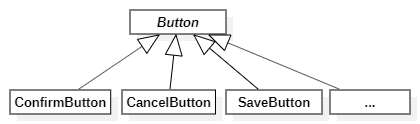
\includegraphics[scale=0.8]{naiveButtons}
\caption{Bottoni naive}
\label{fig:naiveButtons}
\end{figure}
\\Quando i bottoni sono tanti però questo porta a dover creare tante sottoclassi e una modifica alla classe padre potrebbe risultare molto costosa.\\
Inoltre se volessimo eseguire la stessa azione di un bottone tramite ad esempio uno shortcut da tastiera dovremmo o copiare il codice del bottone nella classe dello shortcut o rendere queste due classi l'una dipendente dall'altra.
\begin{figure}[h!]
\centering
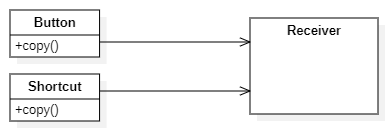
\includegraphics[scale=0.8]{commandNaive.png}
\caption{Copia naive}
\label{fig:naiveCopy}
\end{figure}

\subsection{Annullare un comando}\label{undo}
Vogliamo anche permettere all'utente di annullare un comando eseguito e ripristinare l'elemento modificato allo stato precedente. Per farlo dobbiamo salvare un istantanea dello stato dell'oggetto prima che il comando venga eseguito. La soluzione naive è quella di lasciare che il comando stesso si occupi di iterare su ogni attributo dell'oggetto per copiare i valori attuali, ma questo potrebbe funzionare solo se la classe dell'oggetto lasciasse accessibili tutti i suoi attributi, e questo non è desiderabile nella maggior parte dei contesti. \\
Inoltre anche se ciò fosse realizzabile, se ad un certo punto la classe venisse modificata, andrebbe riaperta anche la classe del comando per aggiornare gli attributi da salvare.

\section{Soluzione}
\subsection{Command pattern}
Invece di lasciare che il componente chiami direttamente i metodi del receiver, il pattern Command suggerisce che queste richieste vengano incapsulate in una classe separata che gestisce le azioni da eseguire. In questo modo il componente non deve conoscere il destinatario della richiesta né come questa viene gestita, ma invoca il comando che si occuperà del resto.
\begin{figure}[h!]
\centering
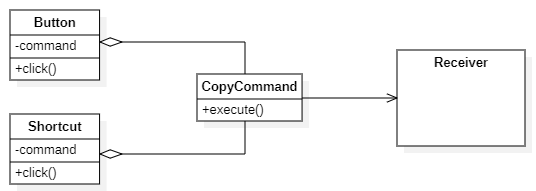
\includegraphics[scale=0.8]{commandBetter.png}
\caption{Copia tramite classe intermedia}
\label{fig:proCopy}
\end{figure}
\newpage
Per completare il pattern basta che tutti i comandi implementino la stessa interfaccia in modo che i componenti non siano accoppiati al comando concreto, in questo modo il comando di ogni componente può essere anche modificato al runtime.
\begin{figure}[h!]
\centering
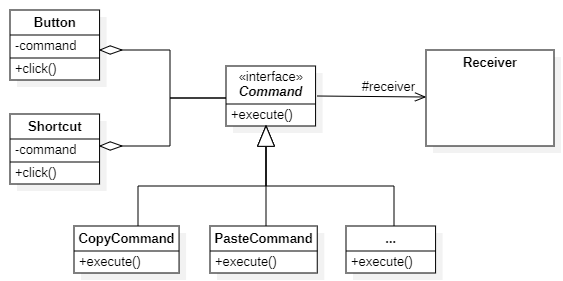
\includegraphics[scale=0.7]{commandPattern.png}
\caption{Command pattern}
\label{fig:commandPattern}
\end{figure}

\subsubsection{Nel progetto}
\textbf{Window} e \textbf{Editor} sono i receivers, i \textbf{Component}s sono gli invokers e \textbf{Command} è l'interfaccia comune ai comandi concreti.\\
Il codice dell'invoker e del comando "Nuovo Editor" sono sotto riportati:\\
\begin{minipage}{\textwidth}
\lstinputlisting[language=Java, caption=Command pattern - Component.java]{code/command/Component.java}
\end{minipage}
\begin{minipage}{\textwidth}
\lstinputlisting[language=Java, caption=Command pattern - Button.java]{code/command/Button.java}
\end{minipage}
\begin{minipage}{\textwidth}
\lstinputlisting[language=Java, caption=Command pattern - Command.java, label={lst:Command.java}]{code/command/Command.java}
\end{minipage}
\begin{minipage}{\textwidth}
\lstinputlisting[language=Java, caption=Command pattern - NewEditorCommand.java]{code/command/NewEditorCommand.java}
\end{minipage}

\subsection{Composite pattern}
L'incapsulamento dei comandi in classi a se stanti permette anche di implementare facilmente la creazione di comandi macro definiti dall'utente tramite il pattern Composite.
\begin{figure}[h!]
\centering
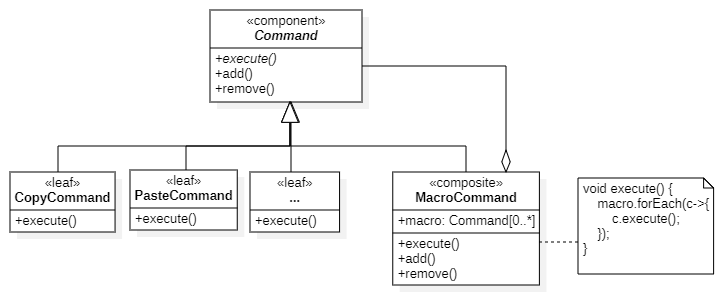
\includegraphics[scale=0.6]{compositePattern.png}
\caption{Composite pattern}
\label{fig:compositePattern}
\end{figure}

\newpage
\subsection{Memento pattern}
Il problema descritto in \ref{undo} deriva dal fatto che cerchiamo di delegare al comando un responsabilità che non gli compete, invece di lasciare tale compito all'oggetto che sicuramente può accedere a tutti i campi da salvare, cioè il proprietario dello stato stesso. \\
Il pattern Memento prevede che lo stato dell'oggetto \emph{originator} venga salvato dentro un oggetto chiamato \emph{memento}, creato dall'originator stesso. Questi snapshots vengono gestiti da un \emph{caretaker}, che vede una interfaccia \emph{ristretta} del memento che può esporre dati non sensibili riguardanti lo snapshot, al contrario dell'originator che ne vede una più \emph{ampia} che gli permette di leggere e ripristinare lo stato salvato.\\
Se più entità hanno uno stato da salvare si può creare una interfaccia comune a tutti i memento in modo che il caretaker possa gestire ogni memento concreto.
\begin{figure}[h!]
\centering
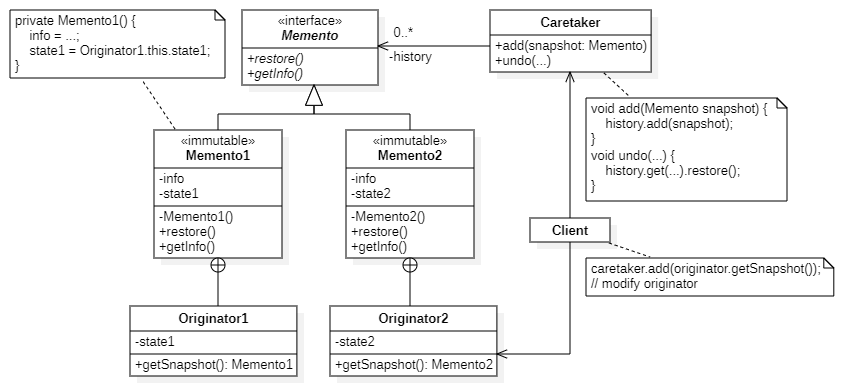
\includegraphics[width=\textwidth]{mementoPattern.png}
\caption{Memento pattern}
\label{fig:mementoPattern}
\end{figure}

\subsubsection{Nel progetto}
\textbf{Window} è il caretaker, \textbf{Editor} è l'originator e i comandi sono il client del diagramma di \hyperref[fig:mementoPattern]{Figura 6}. Sono presenti comandi che non modificano lo stato dell'Editor come \textbf{CopyCommand}, al contrario di altri come \textbf{CutCommand} che per questo chiedono il salvataggio di uno snapshot prima della modifica.\\
Questo caso d'uso è realizzato dal seguente codice (i comandi estendono Command visto in \hyperref[lst:Command.java]{Code 3}):\\
\begin{minipage}{\textwidth}
\lstinputlisting[language=Java, caption=Memento pattern - CutCommand.java]{code/memento/CutCommand.java}
\end{minipage}
\begin{minipage}{\textwidth}
\lstinputlisting[language=Java, caption=Memento pattern - UndoCommand.java]{code/memento/UndoCommand.java}
\end{minipage}
\begin{minipage}{\textwidth}
\lstinputlisting[language=Java, caption=Memento pattern - Window.java]{code/memento/Window.java}
\end{minipage}
\begin{minipage}{\textwidth}
\lstinputlisting[language=Java, caption=Memento pattern - Editor.java]{code/memento/Editor.java}
\end{minipage}

\subsection{Facade pattern}
Per semplificare l'utilizzo dell'applicazione è stata creata una \emph{facciata} che permette al client di accedere alle funzionalità dei sottosistemi senza che esso ne conosca l'architettura sottostante o le dipendenze, che vengono invece installate dalla facciata.
Il client quindi avanza richieste alla facciata che provvede a reindirizzarle alle classi competenti.
\begin{figure}[h!]
\centering
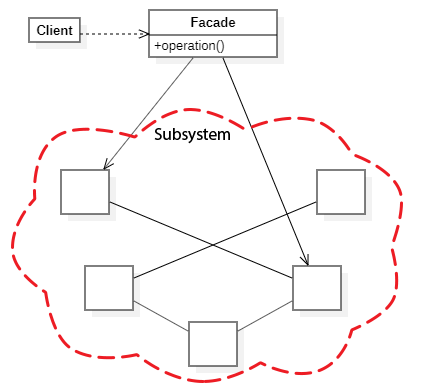
\includegraphics[scale=0.5]{facadePattern.png}
\caption{Facade pattern}
\label{fig:facadePattern}
\end{figure}

\subsubsection{Nel progetto}
Si riporta il codice per il caso d'uso in cui il client vuole scrivere sull'editor attivo e creare una macro:\\
\begin{minipage}{\textwidth}
\lstinputlisting[language=Java, caption=Facade pattern - AppFacade.java]{code/facade/AppFacade.java}
\end{minipage}
\begin{minipage}{\textwidth}
\lstinputlisting[language=Java, caption=Facade pattern - Client.java]{code/facade/Client.java}
\end{minipage}

\newpage
\section{Progetto completo}
Il progetto simula un editor di testo con comandi di \emph{Copia}, \emph{Taglia}, \emph{Incolla}, \emph{Undo} e \emph{Crea nuovo editor} attivabili da \emph{Bottoni} e \emph{Shortcuts}, con la possibilità di creare macro che eseguono più comandi uno dopo l'altro.\\
Il codice completo è accessibile su GitHub al seguente link: \url{https://github.com/marcodiri/progettoSWE2020}

\subsection{Partecipanti}
\textbf{AppFacade} si occupa di installare le dipendenze necessarie e fornisce al client i metodi utili per l'utilizzo dell'applicazione. \\
\textbf{CommandManager} è responsasbile di istanziare i comandi e di passarne i loro riferimenti al richiedente. \\
\textbf{Window} è il \emph{Receiver} del pattern Command e il \emph{Caretaker} del pattern Memento. Ogni window ha il proprio ComponentManager e fornisce una sorta di interfaccia per i comandi che possono richiederle un componente già istanziato o di istanziarne uno nuovo. Mantiene una storia di memento in modo da poter chiedere al componente di ripristinare uno stato precedente.\\
\textbf{ComponentManager} è responsabile di instanziare i componenti su richiesta della Window e gestisce il loro ciclo di vita. Dialoga con il CommandManager per recuperare i comandi da attaccare ai componenti. \\
\textbf{Component} generalizza i componenti dell'applicazione quali bottoni, shortcut e editor.
\textbf{Button}, \textbf{Shortcut} componenti che invocano i comandi.\\
\textbf{Editor} è il \emph{Receiver} del pattern Command e l'\emph{originator} del pattern Memento. Riceve istruzioni dai comandi su come modificare il suo stato. Mantiene lo stato da salvare che in questo caso è il testo, la posizione del cursore e la larghezza della selezione.\\
Contiene i metodi per generare il suo snapshot.\\
\textbf{Memento} è l'interfaccia comune a tutti i memento concreti. Permette di generalizzare i memento in modo che il caretaker possa gestire una collezione composta da tutti i tipi di memento. \\
\textbf{EditorMemento} è il \emph{memento} del pattern Memento. È una classe annidata di Editor che è l'unico capace di istanziarla. Espone dati non sensibili riguardanti lo snapshot come il Timestamp, mentre lo stato salvato non può essere letto o modificato da elementi esterni. È immutabile.\\
\textbf{Command} è il \emph{Component} del pattern Composite. È referenziato da bottoni e shortcut secondo il pattern Command. È una classe astratta che generalizza i vari comandi concreti.\\
\textbf{MacroCommand} è il \emph{Composite} del pattern Composite. Permette di aggregare comandi concreti.\\
\textbf{CutCommand} è una \emph{Leaf} del pattern Composite. È un comando concreto della applicazione insieme agli altri che estendono Command che viene chiamato da un bottone o shortcut. Prima di modificare il receiver, ne chiede uno snapshot che verrà salvato nel caretaker, in modo che le sue azioni possano essere annullate.

\newpage
\newgeometry{left=1in,right=1in,top=0in,bottom=1in}
\begin{landscape}
\begin{figure}[h!]
\centering
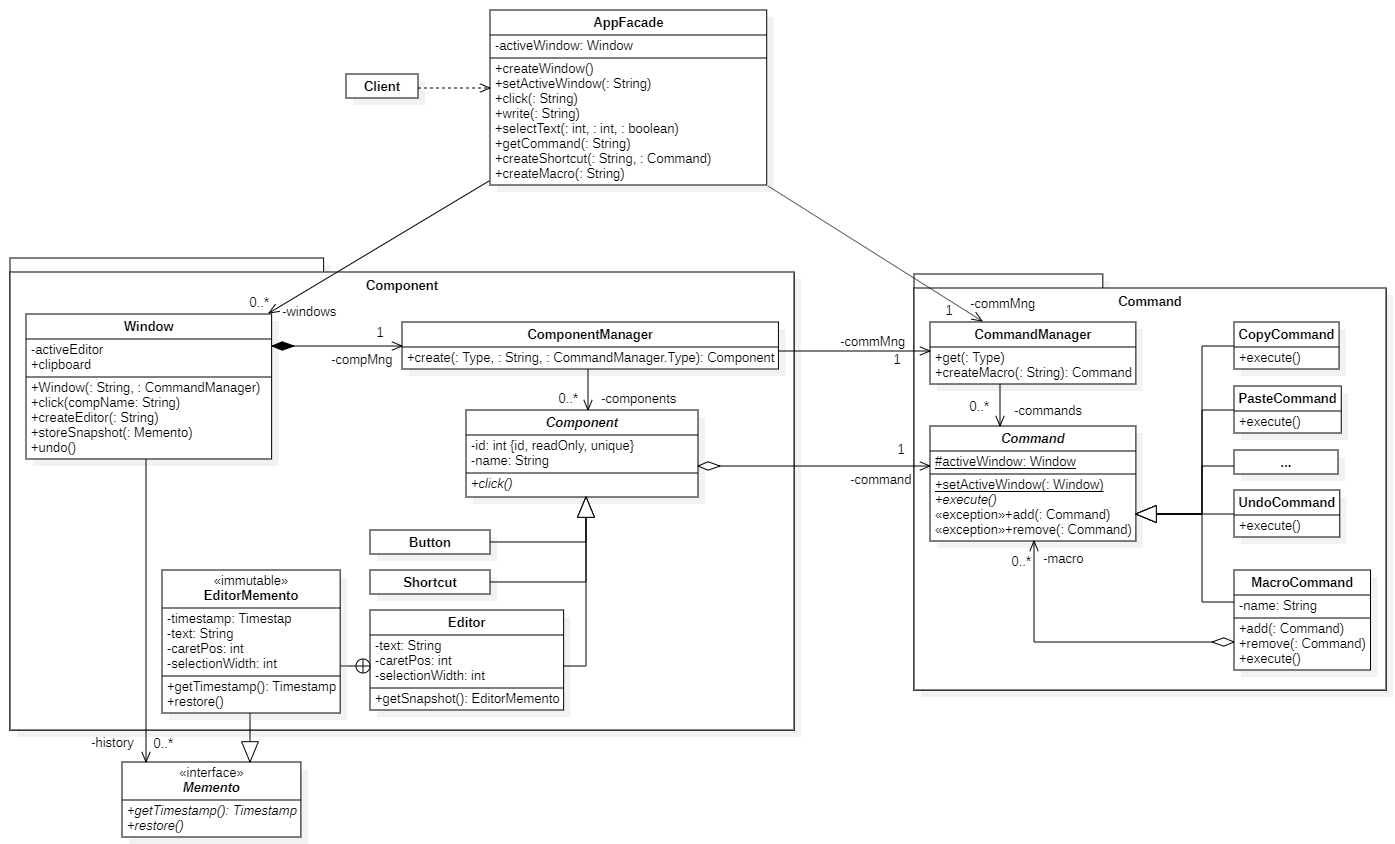
\includegraphics[scale=0.5]{project.png}
\caption{Class diagram progetto}
\label{fig:project}
\end{figure}
\end{landscape}
\restoregeometry

\subsection{Collaborazione}
La collaborazione tra i vari componenti è mostrata di seguito con un esempio in cui si vuole tagliare del testo da un editor e poi ripristinarlo con il comando di undo.
\begin{figure}[h!]
\centering
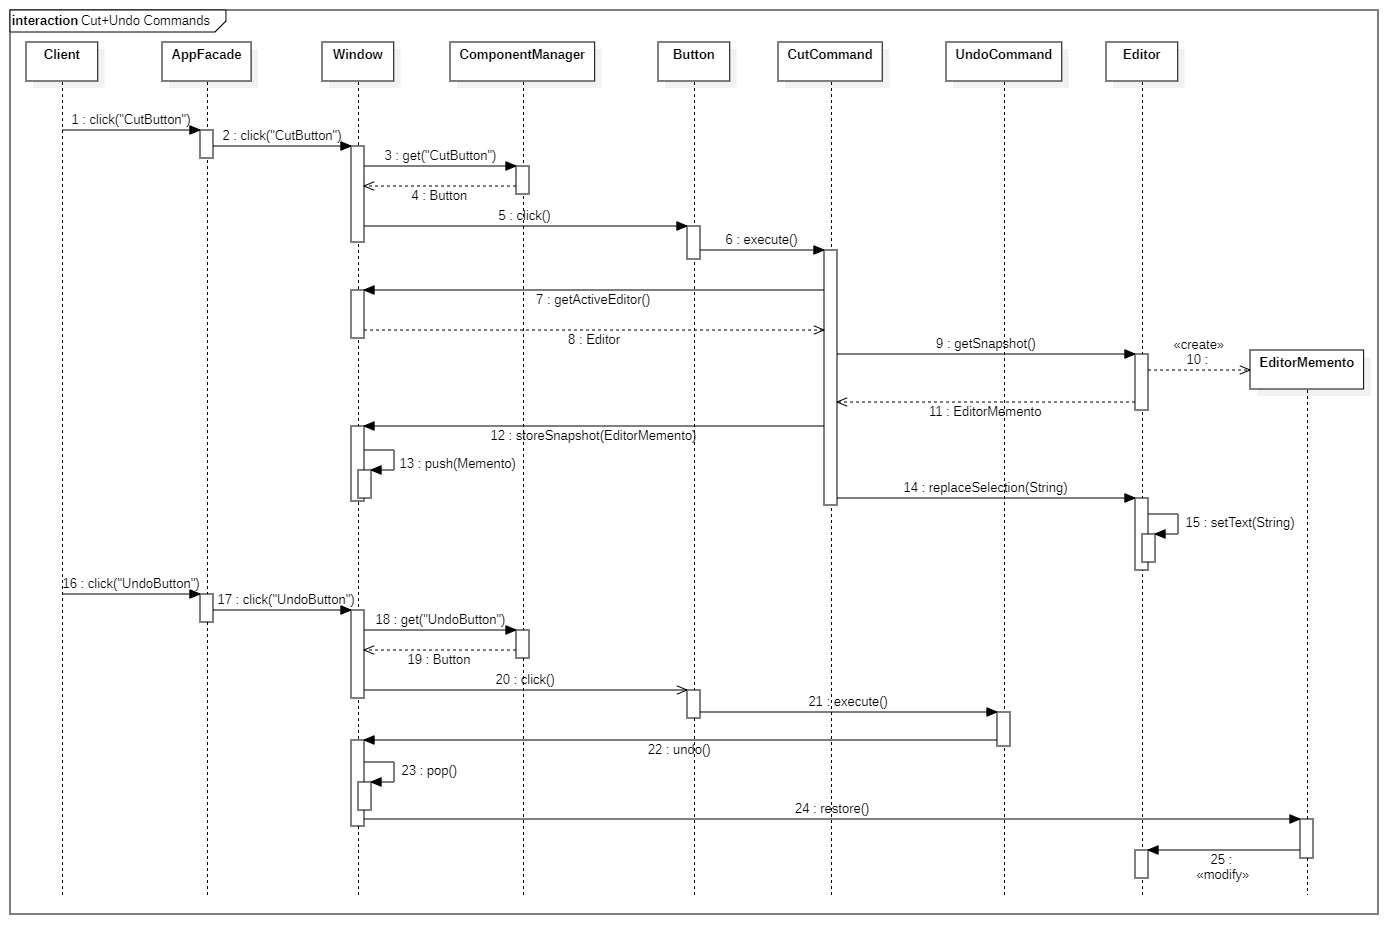
\includegraphics[width=\textwidth]{sequenceDiagram.png}
\caption{Sequence diagram CutCommand + UndoCommand}
\label{fig:lifecycleCutUndo}
\end{figure}

\newpage
\section{Tests}
Si riporta di seguito il codice dei test sui vari componenti con relativo output.\\
\textcolor{firebrick}{N.B. i campi privati vengono testati tramite \emph{reflection}, il cui codice viene omesso per semplicità. Nei vari test saranno quindi presenti campi normalmente non accessibili dal client. Per conoscere il loro ruolo è possibile consultare il class diagram di \hyperref[fig:project]{\color{firebrick}Figura 8}, saranno comunque brevemente descritti ove necessario.}\\
Tutti i test sono preceduti da una inizializzazione \\
\begin{minipage}{\textwidth}
\lstinputlisting[language=Java]{code/tests/before.java}
\end{minipage}

\subsection{Test Command pattern}
Si verifica che sia il bottone che lo shortcut per creare un nuovo Editor abbiano un riferimento alla stessa istanza del comando.\\
\texttt{components} è un campo di \textbf{CommandManager} ed è la collezione dei \textbf{Component} presenti nella \textbf{Window} attiva \\
\begin{minipage}{\textwidth}
\lstinputlisting[language=Java]{code/tests/testCommandPattern.java}
\end{minipage}
\subsubsection{Output}
\begin{figure}[H]
\centering

\includegraphics[width=\textwidth]{tests/testCommandPattern.png}
\caption{Command pattern test output}
\label{fig:testCommandPatternOutput}
\end{figure}

\subsection{Test comando Nuovo Editor}
Si verifica che con il comando Nuovo Editor venga creato correttamente un nuovo Editor e salvato nella lista dei componenti della finestra attiva.\\
\texttt{app.click(nomeComponente)} simula il click dell'utente su un componente della GUI, ad esempio sul bottone chiamato "NewEditorButton". In questo caso il bottone invoca il comando \textbf{NewEditorCommand} che crea un nuovo \textbf{Editor} nella finestra attiva che viene settato come \texttt{activeEditor}.\\
\texttt{activeWindow} è un campo di \textbf{AppFacade} ed è la finestra attiva tra quelle aperte.\\
\texttt{getActiveEditor()} è un metodo di \textbf{Window} che ritorna l'Editor attivo tra quelli presenti nella finestra.\\
\begin{minipage}{\textwidth}
\lstinputlisting[language=Java]{code/tests/testNewEditorCommand.java}
\end{minipage}
\subsubsection{Output}
\begin{figure}[H]
\centering

\includegraphics[width=\textwidth]{tests/testNewEditorCommand.png}
\caption{NewEditor command test output}
\label{fig:testNewEditorCommandOutput}
\end{figure}
\VerbatimInput{code/tests/output/testNewEditorCommand.txt}

\subsection{Test comando Taglia}
Il comando Taglia è reversibile quindi si controlla che richieda uno snapshot dell'Editor prima di modificarlo.\\
\texttt{app.selectText(caretPos, selectionWidth, toRight)} simula una selezione del testo presente nell'Editor attivo. Il testo così selezionato sarà quello tagliato dal comando Taglia.\\
\texttt{history} è un campo di \textbf{Window} ed è lo stack dei vari snapshots richiesti dai comandi.\\
\begin{minipage}{\textwidth}
\lstinputlisting[language=Java]{code/tests/testCutCommand.java}
\end{minipage}
\subsubsection{Output}
\begin{figure}[H]
\centering

\includegraphics[width=\textwidth]{tests/testCutCommand.png}
\caption{Cut command test output}
\label{fig:testCutCommandOutput}
\end{figure}
\VerbatimInput{code/tests/output/testCutCommand.txt}

\subsection{Test comando Undo}
Viene prima richamato il test precedente per poi testare il comando Undo.\\
Si verifica che lo stack degli snapshots sia svuotato e che il testo tagliato venga ripristinato nell'Editor.\\
\begin{minipage}{\textwidth}
\lstinputlisting[language=Java]{code/tests/testUndoCommand.java}
\end{minipage}
\subsubsection{Output}
\begin{figure}[H]
\centering

\includegraphics[width=\textwidth]{tests/testUndoCommand.png}
\caption{Undo command test output}
\label{fig:testUndoCommandOutput}
\end{figure}
\VerbatimInput{code/tests/output/testUndoCommand.txt}

\subsection{Test creazione ed esecuzione comando macro}
Si verifica che il comando creato con \texttt{app.createMacro(name)} venga salvato nella lista dei comandi presente in \textbf{CommandManager} \texttt{commMng} e che venga correttamente collegato allo shortcut definito dall'utente.\\

\lstinputlisting[language=Java]{code/tests/testMacroCommand.java}

\subsubsection{Output}
\begin{figure}[H]
\centering

\includegraphics[width=\textwidth]{tests/testMacroCommand.png}
\caption{Macro command test output}
\label{fig:testMacroCommandOutput}
\end{figure}
\VerbatimInput{code/tests/output/testMacroCommand.txt}

\end{document}
